\subsection{The Model View Controller Pattern}
\label{model_view_controller_pattern_section}

After having had a closer look at common design patterns for persistence and
communication, this section finally considers the so called \emph{Frontend} of
an application which is mostly realized in form of a graphical user interface.\\
Nowadays, the well-known \emph{Model View Controller} design pattern
(figure \ref{modelviewcontroller_figure}) is used by nearly all standard applications.
Its principle is to have the \emph{Model} holding domain data, the \emph{View}
accessing and displaying these data and the \emph{Controller} providing the workflow
of the application by handling any signals (actions) appearing on the view.

\begin{figure}[ht]
    \begin{center}
       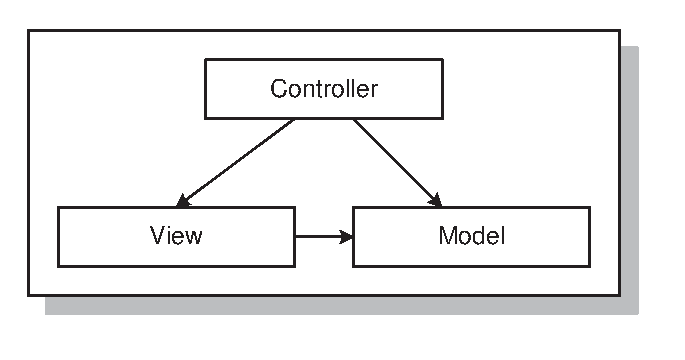
\includegraphics[scale=0.7]{images/model_view_controller_pattern.eps}
       \caption{Classical MVC}
       \label{modelviewcontroller_figure}
    \end{center}
\end{figure}

Since the view (graphical user interface) serves as means of communication between
a software system (application) and its user (Human Being as system), the view
is in fact just another type of communication model that should be assembled
by a special translator.\\
Because there are many ways in which domain data can be displayed, different
user interfaces can exist. Each of them has to have its very own translator item
that knows how to map data both ways, from the domain model to the user interface
model and vice-versa.
